\documentclass[aps,prb,10pt,showkeys,letterpaper,notitlepage,twocolumn]{revtex4-1}
\usepackage{graphicx}
\usepackage{amsmath}
\usepackage[caption=false]{subfig}
\usepackage[colorlinks=true,citecolor=red]{hyperref}

\graphicspath{{.}{figures/}}

\begin{document}

\title{\emph{Ab initio} Modeling of Optical Functions after Strain Wave
Perturbation for Defect Detection}
\author{Sean M. Anderson}\email{sma@cio.mx}
    \affiliation{Centro de Investigaciones en \'Optica, 
                Le\'on, Guanajuato, M\'exico}
\author{Bernardo S. Mendoza}%\email{bms@cio.mx}
    \affiliation{Centro de Investigaciones en \'Optica, 
                Le\'on, Guanajuato, M\'exico}
\author{Ram\'on Carriles}%\email{ramon@cio.mx}
    \affiliation{Centro de Investigaciones en \'Optica, 
                Le\'on, Guanajuato, M\'exico}
\date{\today}

\begin{abstract}
We model the change in the linear optical functions due to the propagation of a
strain wave through a crystalline slab. Defects in the slab are introduced by
arbitrarily displacing one of the atomic layers. The perturbing wave is assumed
to be produced by laser light absorption; the properties of the propagating wave
are explicitly related to the laser and material properties. We apply this model
to a Si(111)(1$\times$1):H slab, and find that the reflectance varies
significantly at photon energies above 2.5\,eV, and that the disordered slab
produces significant changes in the reflectance when compared to the unperturbed
slab. We then induce a defect layer in the slab by uniformly translating an
atomic layer. As the strain wave passes through the material, the behavior of
the calculated reflectance difference spectrum changes according to the defect
layer, allowing us to discern the depth of the defect.
\end{abstract}

\keywords{reflectance spectroscopy, atomic disorder, strain wave, surface, depth
probing}

\maketitle

%%%%%%%%%%%%%%%%%%%%%%%%%%%%%%%%%%%%%%%%%%%%%%%%%%%%%%%%%%%%%%%%%%%%%%%%%%%%%%%%
%%%%%%%%%%%%%%%%%%%%%%%%%%%%%%%%%%%%%%%%%%%%%%%%%%%%%%%%%%%%%%%%%%%%%%%%%%%%%%%%

\section{Introduction}\label{sec:intro}

Defect characterization and profiling techniques in solid materials are becoming
increasingly relevant, coinciding with the many new advances in micro- and
opto-electronics. It is therefore desirable to develop techniques capable of
non-destructive and \emph{in-situ} characterization; particularly, optical
methods have a strong background of applications in this area. These
developments require better theoretical models to understand the experimental
observations. \emph{Ab initio} calculations have been used to obtain optical
properties of materials under strain or with defects. With current computational
systems the calculations from surface or bulk regions are both efficient and
numerically accurate \cite{hoganPRB98, palummoPRB99, hoganPRB03, mendozaPRB06,
palummoPRB09, hingerlASS01}.

Experimentally, pump-probe techniques \cite{thomsenPRL84, thomsenPRB86,
grahnJQE89, linJAP91, pfeiferPRL92} have been widely used to measure and
characterize buried defects and interfaces. In these experiments, at least two
laser beams with different intensities, typically sub-picosecond in duration,
are incident on the sample with a temporal delay. The more intense pump beam is
used to excite the sample, while the weaker probe beam (split off from the pump
beam, or an independent synchronized beam) is used to sense the effect of the
pump on the material. The temporal delay is controlled with a translational
stage and can be as short as a few femtoseconds.

Among these techniques, coherent acoustic phonon (CAP) spectroscopy (also known
as picosecond ultrasonics) is well established. In this case, the pump is
absorbed by the sample and induces a traveling strain wave that locally modifies
the optical properties as it traverses the material. The probe pulse senses the
induced changes and therefore provides information about the local environment
inside the sample. Due to its flexibility, the CAP method has been used to study
many sample attributes, such as structural properties of a wide range of
materials \cite{limAPL03, bozovicPRB04, matsudaPRL04, rossignolPRL05, parkPRB05,
wuAPL06, millerPRB06, wenAPL07, xuPSSC08, hudertJAP08, ruelloPRB09,
babilottePRB10, ruelloAPL12, chenAPL12}, characterization of thin films
\cite{gusevJAP11, matsudaJOSAB02}, determination of elasto-mechanical and
optical properties \cite{grahnAPL88a, grahnAPL88b, rossignolPRL05, millerPRB06,
xuPSSC08, taneiPRL08, qiPRB10}, low-frequency phonon dispersion and attenuation
\cite{zhuPRB91, dalyPRB09}, roughness of buried interfaces \cite{tasAPL98},
inhomogeneities in disordered films \cite{gusevJAP11}, doping profiles
\cite{hudertJAP08}, lattice defects \cite{steigerwaldJAP12, steigerwaldAPL09,
gregoryAPL12, baydinAPLP16}, and shear strain waves using time-resolved
polarization measurements \cite{mounierEPJST08, mounierOE10}. Recently, the
development of 2-dimensional materials and membranes has introduced new
challenges related to the characterization of their properties. CAP has begun to
be applied to thin films and free standing membranes \cite{linJPD16, hePRB17},
magnetic nano-films \cite{linnikPS17}, nanoparticles \cite{baldiniNL18}, and van
der Waals nanolayers \cite{greenerPRB18}; however, it is necessary to refine the
current theoretical models to better understand how the presence of defects
alters the material properties.
 
In a previous work \cite{andersonPSSB18}, we presented a simple \emph{ab initio}
model to study how the displacement of a single atomic layer inside a material
affected its linear optical properties. We applied the model to a
Si(111)(1$\times$1):H slab and found that the predicted reflectance changes were
within the sensitivity range of lock-in techniques. In this work, we simulate
the propagation of a strain wave inside a material and the related atomic
displacement induced by the traveling wave, and calculate the resulting change
in the dielectric function. The goal of this work is twofold: first, to develop
a realistic model of strain waves, and how they perturb a given material at the
atomic level; second, to apply the developed model towards the detection of
buried defects or interfaces. Although our calculations are done using an
analytical form of a CAP strain wave, our model is valid for any type of
deformations induced in the bulk atomic positions.

This paper is organized as follows. In Sec. \ref{sec:theory}, we present the
relevant equations and theory that characterize both the strain wave and the
reflectance difference spectrum. In Sec. \ref{sec:results}, we present and
analyze the calculated reflectance from probing a Si(111)(1$\times$1):H surface
as a test case, exploring several cases including buried defects. Finally, we
list our conclusions and final remarks in Sec. \ref{sec:conc}.

%%%%%%%%%%%%%%%%%%%%%%%%%%%%%%%%%%%%%%%%%%%%%%%%%%%%%%%%%%%%%%%%%%%%%%%%%%%%%%%%
%%%%%%%%%%%%%%%%%%%%%%%%%%%%%%%%%%%%%%%%%%%%%%%%%%%%%%%%%%%%%%%%%%%%%%%%%%%%%%%%

\section{Theory}\label{sec:theory}

%%%%%%%%%%%%%%%%%%%%%%%%%%%%%%%%%%%%%%%%%%%%%%%%%%%%%%%%%%%%%%%%%%%%%%%%%%%%%%%%

\subsection{Strain wave generation from CAP pulses}

We previously developed a simple proof-of-concept model \cite{andersonPSSB18}
where individual atomic layers were uniformly translated up or down by a given
percentage. These movements yielded a clear difference in reflectivity between
the perturbed and unperturbed slabs, with discernible changes when either
diagonal or vertical bonds underwent the deformation; specifically, elongation
of the diagonal bonds (compression of the vertical bonds) leads to an increase
in the reflectance difference spectrum.

Our goal is now to extend and improve upon our previous work, and create a far
more realistic strain wave model that is capable of detecting defects within a
given slab. As a starting point, Ref. \onlinecite{wuPRB07} extends upon
previously developed analytical models for strain wave generation from CAP
\cite{thomsenPRB86}, and demonstrates that the electronic stress plays a large
role in inciting the CAP pulse. The produced strain in the $z$ direction,
$\eta_{zz}$, can be approximated in simple analytical form as \cite{wuPRB07}
\begin{equation}\label{eq:strain}
\eta_{zz}(z,t) = -A e^{-\alpha|z - v_{s}t|} \,\mathrm{sgn}(z - v_{s}t),
\end{equation}
where $\alpha$ is the absorption coefficient of the material at the pump beam
energy, and $v_{s}$ is the longitudinal sound velocity. The dimensionless
pre-factor $A$ determines the strength of the strain wave and is given by
\begin{equation}\label{eq:prefactor}
\begin{split}
A = \frac{\alpha(1 - R_{\mathrm{pump}})Q}
         {2E_{\mathrm{pump}}\rho v_{s}^{2}}
\bigg[
&- \left(d_{c} + d_{v}\right)\\
&+ \frac{3B\beta}{C_{V}}\left(E_{\mathrm{pump}} - E_{g}\right)
\bigg],
\end{split}
\end{equation}
where $R_{\mathrm{pump}}$, $Q$, and $E_{\mathrm{pump}}$ are the reflectance,
fluence, and photon energy of the pump beam, $E_{g}$ is the band gap energy,
$\rho$ is the mass density, $d_{c}$ and $d_{v}$ are the electron and hole
deformation potentials, $B$ is the bulk modulus, $\beta$ is the linear thermal
expansion coefficient, and $C_{V}$ is the specific heat per unit volume. The
produced strain in Eq. \eqref{eq:strain} is related to the lattice displacement
$u(z,t)$ as
\begin{equation*}
\eta_{zz}(z,t) = \frac{\partial u(z,t)}{\partial z};
\end{equation*}
after integrating with respect to $z$, we finally obtain
\begin{equation}\label{eq:displacement}
\begin{split}
u(z,t)
&= -\frac{A}{2 \alpha}\bigg(
e^{\alpha (-z + v_{s}t)}
\Big[\,\mathrm{sgn}(-z + v_{s}t) - 1\Big]\\
&\hspace{1.05cm}+
e^{\alpha (+z - v_{s}t)}
\Big[\,\mathrm{sgn}(+z - v_{s}t) - 1\Big]
\bigg).
\end{split}
\end{equation}
Fig. \ref{fig:pulse} depicts the calculated strain and displacement profiles
obtained from Eqs. \eqref{eq:strain} and \eqref{eq:displacement} for a fixed
time $t$ as functions of the distance traveled, into the material, $z-v_{s}t$.
These curves are produced using physical parameters for silicon (see Tables
\ref{tab:constants} and \ref{tab:params}). As the pulse travels through the
material, the atoms will be displaced according to Eq. \eqref{eq:displacement};
thus, careful selection of the beam characteristics will greatly affect how much
the (and how many) atoms are displaced from their equilibrium positions.

\begin{figure}[t]
\centering
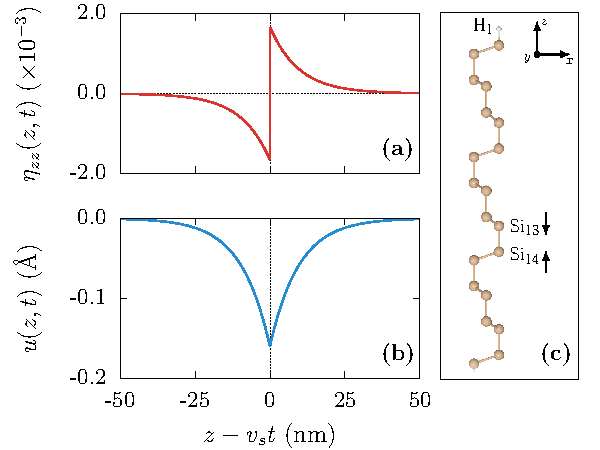
\includegraphics[width=\linewidth]{fig01}
\caption{Time-snapshot of the \textbf{(a)} strain and \textbf{(b)} displacement
profiles (as functions of the distance traveled) of a CAP pulse using parameters
for silicon (Tables \ref{tab:constants} and \ref{tab:params}). These plots were
calculated for a fluence $Q = 0.3$\,mJ/cm$^{2}$, a pump photon energy
$E_{\mathrm{pump}} = 3.54$\,eV which corresponds to an absorption coefficient
$\alpha = 1.04\times10^{6}$\,cm$^{-2}$. \textbf{(c)} Cartoon representation of
the slab unit cell, with two Si labeled atoms that will be moved in the
direction indicated to create buried defect layers. The $x$ and $y$ axes are
taken along the [$11\bar{2}$] and [$1\bar{1}0$] directions, respectively.}
\label{fig:pulse}
\end{figure}

\begin{table}[b]
\caption{Material constants for silicon.}
\label{tab:constants}
\begin{ruledtabular}
\begin{tabular}{ l l l }
Parameter                               & Sym.      & Value                           \\
\hline
Longitudinal sound velocity             & $v_{s}$   & 8433\,m\,s$^{-1}$\cite{sisound} \\
Mass density                            & $\rho$    & 2.3296\,g\,cm$^{-3}$            \\
Bulk modulus                            & $B$       & 98\,GPa\cite{hopcroftJMS10}     \\
Thermal expansion coefficient           & $\beta$   & $2.56\times10^{-6}$\,K$^{-1}$   \\
Electron deformation potential          & $d_{c}$   & 9.5\,eV\cite{lundstrom2000}     \\% Table 2.1, p. 114
Hole deformation potential              & $d_{v}$   & 5.0\,eV\cite{lundstrom2000}     \\% Table 2.1, p. 114
Direct Band gap                         & $E_{g}$   & 3.4\,eV\cite{landolt}           \\
Specific heat per unit volume           & $C_{V}$   & 1.63072\,J\,cm$^{-3}$\,K$^{-1}$ \\
\end{tabular}
\end{ruledtabular}
\end{table}

\begin{table}[t]
\caption{Beam and wavelength-dependent parameters used throughout this work,
unless stated otherwise.}
\label{tab:params}
\begin{ruledtabular}
\begin{tabular}{ l l l }
Parameter               & Sym.                  & Value                          \\
\hline
Pump beam fluence       & $Q$                   & 0.5861\,mJ\,cm$^{-2}$          \\
Pump beam energy        & $E_{\mathrm{pump}}$   & 3.54\,eV                       \\
Pump beam reflectance   & $R_{\mathrm{pump}}$   & 0.56538                        \\
Pump beam absorption    & $\alpha$              & $1.04\times10^{-6}$\,cm$^{-1}$ \\
\end{tabular}
\end{ruledtabular}
\end{table}

%%%%%%%%%%%%%%%%%%%%%%%%%%%%%%%%%%%%%%%%%%%%%%%%%%%%%%%%%%%%%%%%%%%%%%%%%%%%%%%%

\subsection{\emph{Ab initio} calculation of the reflectance}

To model a semi-infinite crystal, we create a slab consisting of $N$ atomic
layers and thickness $D$ inside of a super-cell of height $L$; this super-cell
includes a vacuum region that is large enough to avoid spurious wavefunction
tunneling into neighboring super-cells \cite{mendozaPRB06}. The slab surface is
parallel to the $xy$ plane. The reflectance difference spectrum $\Delta R$ is
defined as \cite{mendozaPRB06}
\begin{equation*}
\Delta R 
= \frac{R_{x}+R_{y}}{2}\bigg|_{\mathrm{unperturbed}}
- \frac{R_{x}+R_{y}}{2}\bigg|_{\mathrm{perturbed}}
,
\end{equation*}
where $R_{\mathrm{a}}$ ($\mathrm{a} = x$ or $y$) is the normal incident
reflectance for linearly polarized light in the $\hat{\mathbf{a}}$ direction. As
explained above, the advancing strain wave will displace the atoms of the slab
away from their equilibrium positions; we calculate $R_{\mathrm{a}}$ for this
perturbed slab and obtain the difference ($\Delta R$) between the reflectance of
the perturbed and unperturbed slabs. $R_{\mathrm{a}}$ can be calculated through
the optical response of the slab system \cite{delsolechap95} as
\begin{equation}\label{eq:Ra}
R_{\mathrm{a}} = 
4\left(\frac{\omega}{c}\right)
\mathrm{Im}
\bigg[
\frac{(D/2)\chi^{\mathrm{aa}}_{sc}(\omega)}
     {\boldsymbol{\chi}^{~}_{b}(\omega)}
\bigg]
,
\end{equation}
where $\omega$ is the angular frequency of the normally incident light impinging
at the slab surface, $c$ is the speed of light, $D/2$ is half of the slab
thickness, $\boldsymbol{\chi}_{sc}(\omega)$ is the linear susceptibility for the
supercell system, and $\boldsymbol{\chi}^{~}_{b}(\omega)$ is the linear
susceptibility of the isotropic bulk crystal.

The linear susceptibility tensor is calculated within the independent-particle
framework as
\begin{equation}\label{eq:chi1}
\chi^{\mathrm{aa}}(\omega) =
\frac{e^{2}}{\hbar}
\int\frac{d\mathbf{k}}{8\pi^{3}}
\sum_{m<n}\frac{2f_{mn}(\mathbf{k})}{W_{nm}(\omega)}
\mathrm{Im}
\left[
v^{\mathrm{a}}_{nm}(\mathbf{k})r^{\mathrm{a}}_{mn}(\mathbf{k})
\right],
\end{equation}
where $v^{\mathrm{a}}_{nm}(\mathbf{k})$ and $r^{\mathrm{a}}_{nm}(\mathbf{k})$
are the matrix elements of the electron velocity and position operators, with
$\mathrm{a,\,b} = x,y$ and $n$, $m$ represent the electronic bands. The
Fermi-Dirac distribution is represented as a Heaviside function,
$f_{n}(\mathbf{k}) = \Theta\left(E_{F} - E_{n}(\mathbf{k})\right)$, where
$E_{F}$ is the Fermi energy, $E_{n} = \hbar \omega_{n}(\mathbf{k})$ is the
energy of the electronic band $n$ at point $\mathbf{k}$ in the irreducible
Brillouin zone, and $f_{mn}(\mathbf{k}) = f_{m}(\mathbf{k}) -
f_{n}(\mathbf{k})$. Lastly, we have
\begin{equation*}\label{eq:wnm}
W_{nm}(\omega) =
(\omega_{nm} - \omega - i\gamma)
(\omega_{nm} + \omega + i\gamma),
\end{equation*}
where $\omega_{nm}(\mathbf{k}) = \omega_{n}(\mathbf{k}) -
\omega_{m}(\mathbf{k})$. Many-body interactions can be included in
$\omega_{nm}(\mathbf{k})$ by making use of the scissors operator. The first
(second) term includes the resonant (nonresonant) terms. $\gamma$ signifies the
adiabatic switching of the interaction, and can also be used to include the
broadening of the electronic levels. The limit of $\gamma\to 0$ leads to the
Dirac delta functions $\delta(\omega_{nm}(\mathbf{k}) - \omega)$ for the
resonant term, and $\delta(\omega_{nm}(\mathbf{k}) + \omega)$ for the
nonresonant term; both are needed to accurately calculate
$\chi^{\mathrm{aa}}(\omega)$ \cite{tancognePRB14}. The bulk susceptibility,
$\boldsymbol{\chi}^{~}_{b}(\omega)$, is obtained by using a bulk unit cell in
Eq. \eqref{eq:chi1}; likewise, $\boldsymbol{\chi}_{sc}(\omega)$ is obtained by
using a supercell, where it must be properly normalized with respect to the
vacuum included in the total supercell height $L$ \cite{tancognePRB15}. Then, we
take $\boldsymbol{\chi}_{sc}(\omega)\to(L/D)\boldsymbol{\chi}_{sc}(\omega)$, so
that even if a larger vacuum region is included, the results remains invariant.

%%%%%%%%%%%%%%%%%%%%%%%%%%%%%%%%%%%%%%%%%%%%%%%%%%%%%%%%%%%%%%%%%%%%%%%%%%%%%%%%

\subsection{Test Case, Computational Details, and Depth probing}

We carry out our study using the Si(111)(1$\times$1):H surface, where the
addition of an H atom at each surface passivates the dangling bond of the ideal
Si(111) bulk and yields an unreconstructed surface with a 1$\times$1 unit cell.
In this work, our surface is represented by a centrosymmetric slab of 98 atomic
layers comprised of 96 Si atoms between two H atoms, one at each surface; the
total height of this slab is $151$\,\r{A}. This number of atoms results in a
total of 193 occupied states (neglecting spin); we can fully describe the
desired spectral energy range by including 107 unoccupied states. The hexagonal
symmetry of this surface is such that $\chi^{xx}_{sc}(\omega) =
\chi^{yy}_{sc}(\omega)$, and thus $R_{x} = R_{y}$.

The self-consistent ground state and the Kohn-Sham states needed to construct
the electron velocity and position matrix elements in Eq. \eqref{eq:chi1}, were
calculated within the DFT-LDA framework using the plane-wave ABINIT code
\cite{gonzeCPS09, abinit} using a planewave basis set with Troullier-Martin LDA
pseudopotentials \cite{troullierPRB91}. Our calculation of
$\chi^{aa}_{sc}(\omega)$ was carried out using the TINIBA code \cite{tiniba}. We
found converged results with 91 \textbf{k}-points in the irreducible Brillouin
zone (equivalent to 1922 \textbf{k}-points when neglecting symmetry relations)
and an energy cutoff of 7 Hartrees. Likewise, 3107 $\mathbf{k}$ points and a
cutoff energy of 10 Ha were used for the bulk
$\boldsymbol{\chi}^{~}_{b}(\omega)$ calculation. A scissors shift of 0.7 eV was
{\color{red}%
used for both the surface and bulk susceptibilities featured in Eq.
\eqref{eq:Ra}, obtained from \emph{ab initio} $G_{0}W_{0}$ calculations
\cite{liPRB10}.
}%
The contribution from the nonlocal part of the pseudopotentials
\cite{andersonPRB15} was carried out using the DP \cite{olevanoDP, reiningEXC}
code with a basis set of 5000 planewaves.

Eqs. \eqref{eq:prefactor} and \eqref{eq:displacement} establish how the physical
parameters of the material, in conjunction with the pump beam properties, are
responsible for determining the strain wave displacement amplitude and width.
Some of these parameters are constants that are specific to the material; for
instance, see Table \ref{tab:constants} for a summary of the physical constants
for silicon. Parameters such as $E_{\mathrm{pump}}$ and $Q$ are determined
solely by the laser system, while $\alpha$ and $R_{\mathrm{pump}}$ are both
material-specific and wavelength-dependent. This gives us flexibility to select
the best parameters for modeling a realistic strain wave that is well-suited for
our sample slab (with the necessary computational expense), while using
real-world beam characteristics that can be found in many modern ultrafast laser
systems. Table \ref{tab:params} summarizes the beam and wavelength-dependent
parameters we used throughout this work, unless stated otherwise.

After selecting the appropriate constants and parameters, we simulate the
traveling strain wave by calculating the atomic displacement from Eq.
\eqref{eq:displacement}. The maximum displacement wave-front travels through the
slab (localized at $v_{s}t$), and the atoms are displaced by the corresponding
amount depending on their distance from the wave-front. In order to minimize the
computation expense, we executed a calculation with the wave-front centered at
the $z$-coordinate of each atomic layer. Therefore, each result presented below
consists of 98 separate calculations, one for each step in the strain wave's
movement through the slab. It is important to note that the constants and
parameters from Tables  \ref{tab:constants} and \ref{tab:params} produce a
strain wave that is wider than our 151\,\r{A}-deep slab; however, as we are
mostly interested in the defect-probing capabilities, the small size of the slab
is not a limitation.

%%%%%%%%%%%%%%%%%%%%%%%%%%%%%%%%%%%%%%%%%%%%%%%%%%%%%%%%%%%%%%%%%%%%%%%%%%%%%%%%
%%%%%%%%%%%%%%%%%%%%%%%%%%%%%%%%%%%%%%%%%%%%%%%%%%%%%%%%%%%%%%%%%%%%%%%%%%%%%%%%

\section{Results}\label{sec:results}

In this section, we will review our calculated results for $\Delta R$ generated
by perturbing the Si(111)(1$\times$1):H test slab with a strain wave generated
with the parameters from Tables \ref{tab:constants} and \ref{tab:params}. We
will consider the upper slab surface at $z = 0$, and the bottom surface at $z =
151$\,\r{A}; while this size is several orders of magnitude smaller than the
samples used in most CAP experiments \cite{steigerwaldAPL09, steigerwaldJAP12,
cuffePRL13, lawlerMRE14}, we are still able to gain insight on the microscopic
perturbations that lead to significant changes in the reflectance difference
spectrum.

\begin{figure}[b]
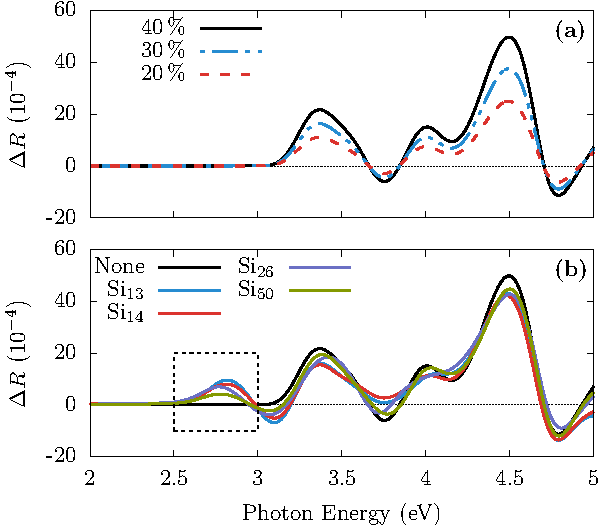
\includegraphics[width=\linewidth]{fig02}
\caption{\textbf{(a)} $\Delta R$ for maximum displacements of 40, 30, and 20\,\%
of the diagonal bond height $H_{d} = 0.784$\,\r{A}, generated with three
different fluence values ($Q = 0.586$, 0.440 and 0.293\,mJ\,cm$^{-2}$).
\textbf{(b)} $\Delta R$ calculated from a max. displacement of 40\,\% of $H_{d}$
for the normal slab and five cases of slabs with defect layers at the atom
indicated in the label for each curve; all curves are produced when the strain
maximum (the wave-front) is at the top surface of the material. The dashed box
highlights the defect peak.}
\label{fig:diffs}
\end{figure}

Fig. \ref{fig:diffs}, panel (a) presents $\Delta R$ generated by the CAP pulse
at the top surface of the slab ($z = 0$) for maximum displacement values of
0.313, 0.235, and 0.157\,\r{A}, which represent 40, 30, and 20\,\% of the
diagonal bond height $H_{d} = 0.784$\,\r{A}. These displacements are generated
using fluence values of $Q = 0.586$, 0.440 and 0.293\,mJ\,cm$^{-2}$,
respectively, and are of the same order as those induced in real samples during
a CAP experiment \cite{lawlerMRE14}, and are large enough to create clear
features in the spectrum, without creating spurious effects from overly
distorted atomic positions. We can see that $\Delta R$ changes monotonically
with the fluence; as the fluence is only limited by the damage threshold of the
sample material, we can essentially select any realistic value that yields
desirable pulse characteristics. Thus, we will use $Q = 0.586$\,mJ\,cm$^{-2}$
(max. displacement of 40\,\% $H_{d}$) for the remainder of this work.

Given that the strain pulse is capable of generating a significant change in the
reflectance, we are now ready to analyze the effect of defects and buried
interfaces on the spectrum. Fig. \ref{fig:diffs}, panel (b) presents $\Delta R$
generated by the strain wave wave-front at the top-most surface atom of a
variety of slabs, with and without defect layers. To identify which atom will be
moved to create a defect layer, we tag each one in consecutive order starting at
the surface, i.e. H$_{1}$ and Si$_{2}$ down to Si$_{97}$ and H$_{98}$. Odd Si
atoms have the vertical bonds going down and the slanted bonds going up, and
vice versa for the even Si atoms; see Fig. \ref{fig:pulse}, panel (c) for a
cartoon representation of the slab. We create the defect layers by moving a
given atom up or down by 0.313\,\r{A} (40\,\% of $H_{d}$); Si$_{13}$ is moved
downwards, while Si$_{14}$, Si$_{26}$, and Si$_{50}$ are moved upwards. The
curve labeled ``None'' (black solid line) is the slab without any defect, the
same shown in panel (a).

Between 3.0--5.0\,eV, $\Delta R$ remains quite similar between the normal and
defective slabs. The spectra is dominated by 2 peaks at around $\sim$3.4\,eV and
$\sim$4.3\,eV, which correspond to the E$_{1}$ and E$_{2}$ critical points of
silicon, with a smaller feature around 4.0\,eV. These peaks mostly retain their
position despite the presence of the defect layers, with small variations in the
peak height. The most interesting feature of the spectra occurs in 2.5--3.0\,eV
energy range, highlighted in the dashed box. A small peak emerges for the
defective slabs that is completely absent from the spectra of the normal slab.
The height of this peak is larger for slabs with the defect layer closer to the
upper surface; likewise, the peak energy position also shifts slightly from
higher energies to lower energies in the same manner. For convenience of
notation, we will call this the defect peak.

\begin{figure}[t]
\centering
\subfloat[Strain wave traveling through a slab with no defect. $\Delta R$ goes
from maximum to minimum, passing through zero at the middle of the slab. The
thin black line indicates the center of the slab at which $\Delta R$ is at a
minimum.\label{fig:depth_normal}]
{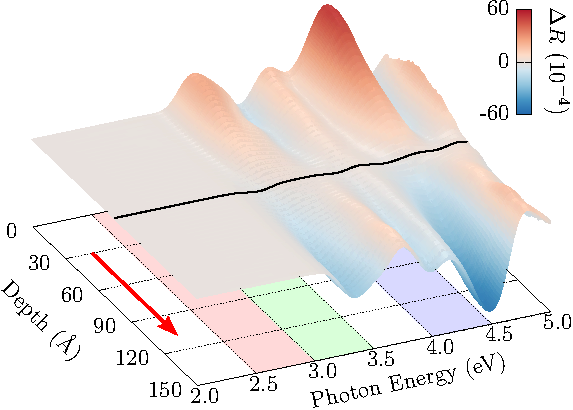
\includegraphics[width=0.95\linewidth]{fig03a}}
\\
\subfloat[Strain wave traveling through a slab with a defect layer at atom
Si$_{50}$. The defect peak goes from positive to negative at the exact position
of the defect layer. The thin black line is a visual aid indicating the depth at
which change in $\Delta R$ occurs due to the defect
layer.\label{fig:depth_defect}] {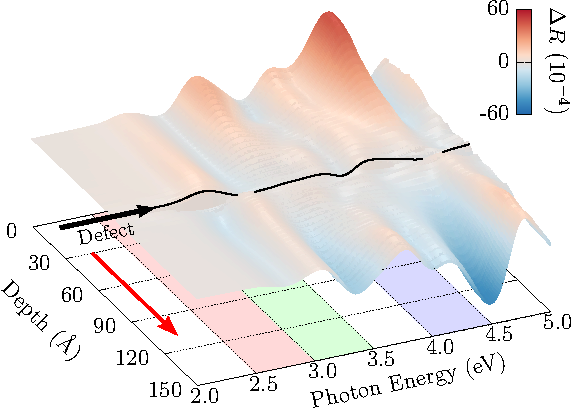
\includegraphics[width=0.95\linewidth]{fig03b}}
\caption{Three-dimensional representation of the reflectivity difference
spectrum ($\Delta R$) as a function of the strain wave depth inside the slab.
The red arrow indicates the direction of propagation of the wave, starting at a
depth of 0 (top surface of the slab) to 151\,\r{A} (bottom surface of the slab).
Colored energy regions will be referred to below.}
\label{fig:depth}
\end{figure}

To explore the depth-probing effects of the strain wave, and the nature of the
defect peak, in Fig. \ref{fig:depth} we present two three-dimensional
representations of $\Delta R$ as the strain wave travels through the slab.
First, Fig. \ref{fig:depth_normal} shows the wave traveling through the normal
slab without defects. $\Delta R$ starts at its maximum value as the wave-front
is located at the material surface. At the middle of the slab, $\Delta R$
essentially goes to zero; after this point, $\Delta R$ goes to negative values,
inverting the shape from the upper half of the slab. This behavior is due to the
fact that our Si(111)(1$\times$1):H slab is centrosymmetric; as the wave reaches
the middle of the slab, the strain wave deforms the upper half in almost exactly
the same way as the lower half. The changes in the reflectance from the upper
half cancel out those from the lower half, and thus $\Delta R$ mostly vanishes.
As shown previously in Fig. \ref{fig:diffs}, the region between 2.5--3.0\,eV is
devoid of any activity.

Second, Fig. \ref{fig:depth_defect} presents the same representation for a slab
with a defect layer present at atom Si$_{50}$, indicated by the black arrow. The
general behavior is similar to the normal slab from Fig. \ref{fig:depth_normal};
however, the defect peak suffers a very marked sign change, from positive to
negative, at the exact position of the defect layer. In fact, we can see a
disturbance across the entire energy range when reaching the defect layer. This
behavior remains consistent for the other defective slabs listed in Fig.
\ref{fig:diffs}. The colored regions on the grid below the plot highlight three
energy ranges; light red for 2.5--3.0\,eV, light green for 3.0--3.5\,eV, and
light purple for 4.0--4.5\,eV, representing the defect peak, the E$_{1}$ peak,
and the E$_{2}$ peak, respectively. In order to better analyze the changes to
$\Delta R$ in the presence of the defect layers, we will study the peaks located
in each of these energy ranges separately.

\begin{figure}[t]
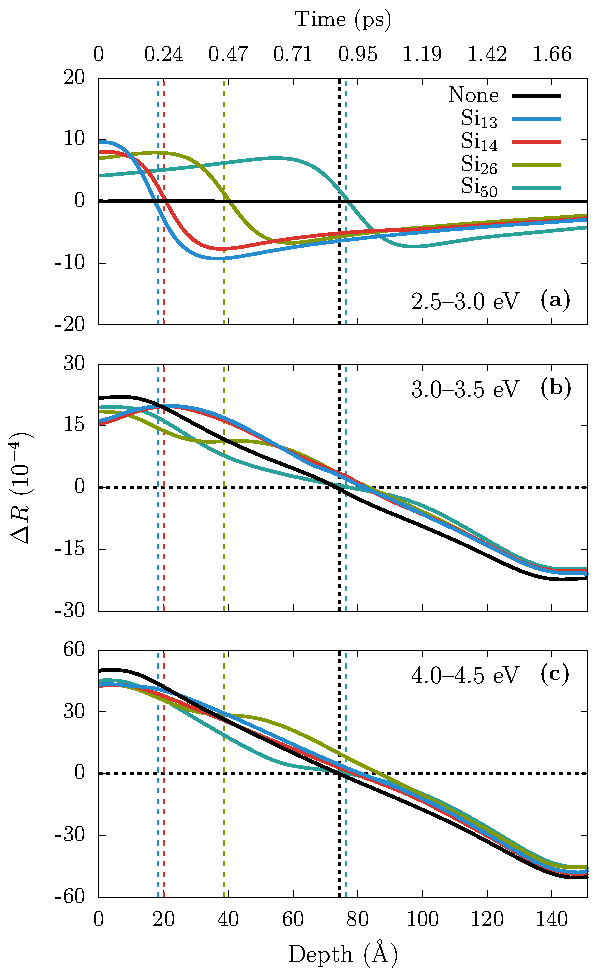
\includegraphics[width=\linewidth]{fig04}
\caption{Peak behavior for the normal and defective slabs, over the \textbf{(a)}
2.5--3.0\,eV, \textbf{(b)} 3.0--3.5\,eV, and \textbf{(c)} 4.0--4.5\,eV regions.
These correspond to the light red, light green, and light purple regions from
Fig. \ref{fig:depth}, respectively. Thin vertical colored dashed lines indicate
the defect depth within the slab. The thick black vertical dashed line
represents the middle of the slab.}
\label{fig:peaks}
\end{figure}

We present the aforementioned peak analysis in Fig. \ref{fig:peaks},
where we plot the intensity of each peak as a function of the strain wave depth
within the slab. Panel (a) depicts the defect peak behavior in the 2.5--3.0\,eV
range (light red region from Fig. \ref{fig:depth}), panel (b) for the E$_{1}$
peak in the 3.0--3.5\,eV range (light green region), and the E$_{2}$ peak in the
4.0--4.5\,eV range (light purple region). We can now clearly see the behavior of
the defect peak for the different defective slabs; when the strain wave reaches
a defect layer, the defect peak goes from positive to negative. The peak
amplitude remains negative after the inversion, and for the remainder of the
strain wave's course through the slab.
Therefore, in order to elucidate the defect layer depth, the measurement would
only have to be taken over the 2.5--3.0\,eV energy range, and when the $\Delta
R$ signal has an abrupt sign change, we know that the strain wave has reached
the defect layer.

Following the same analysis for the E$_{1}$ and E$_{2}$ peaks (panels (b) and
(c)), we see that the induced behavior is not nearly as obvious as for the
defect peak. For the slab with the Si$_{26}$ defect layer, there is a small dip
in the intensity occurring for both peaks before the reaching the defect layer.
Likewise, both peaks have a similar amplitude dip for the Si$_{13}$ and
Si$_{14}$ defective slabs. Interestingly, the places where amplitude of the
E$_{1}$ peak from the defective slabs crosses over the curve representing the
normal slab (black curve) is quite close to the actual defect layer locations.
In other words, the magnitude of the E$_{1}$ peak increases after a defect
layer, when compared directly to the same peak produced in the normal slab.
However, this difference is relatively small and may not be distinct enough to
be measured; also, this behavior is not as strictly followed for the E$_{2}$
peak. Lastly, the slab with the Si$_{50}$ defect layer follows similar trends,
but since the defect is located at the very center of the slab, the changes are
more gradual and are quite close to the normal slab. However, the inflection
point of the curve does indeed indicate the exact location of the defect layer.

These results are consistent with our previous work \cite{andersonPSSB18}. In
particular, defect layers leading to elongated diagonal bonds (corresponding to
upward displacement of even Si atoms, or downward displacement of odd Si atoms)
yield an increase in $\Delta R$ precisely around the same energy energy range
($>2.5$\,eV) as the defect peak reported here. If we consider the response of
the bonds as linear harmonic oscillators, an electron in an elongated bond will
have a looser confinement compared to a compressed bond. The electron potential
for the elongated bond will have a lower curvature, implying that the resonant
frequency (proportional to the curvature) will be lower; thus, the elongated
bond has a higher polarizability which leads to a larger $\Delta R$.

We can further our understanding of these results from a different perspective,
by calculating the dimensionless planar-integrated electron density
\cite{mendozaPRB06},
\begin{equation*}
\rho_{n\mathbf{k}}(z) = L \int |\psi_{n\mathbf{k}}(\mathbf{r})|^{2} \,dx\,dy,
\end{equation*}
for the $n$th valence band and $\mathbf{k}$-vector that contribute to a given
resonance in $\chi^{aa}$ that originates the peaks in $\Delta R$. $L$ is the
total height of the slab, from top surface to bottom surface. For the slab with
a defect at Si$_{13}$, the defect peak at 2.8 eV (dashed box in panel (b) of
Fig. \ref{fig:diffs}) corresponds to $\mathbf{k} = (0.032\,\hat{x} +
0.055\,\hat{y})$\,\r{A}$^{-1}$. Likewise, we can analyze the peak at 4.4 eV for
the relaxed slab (no defect) that corresponds to $\mathbf{k} = (0.062\,\hat{x} +
0.110\,\hat{y})$\,\r{A}$^{-1}$. For both the relaxed and defective slabs, $n =
193$ which corresponds to the topmost valence band.

Using the aforementioned values, we present the electron density as a function
of depth in Fig. \ref{fig:defect}. We see that for the relaxed structure,
$\rho_{n\mathbf{k}}(z)$ is a periodic, symmetric function that grows towards the
center of the slab, which is consistent with the ordered and centrosymmetric
nature of the atomic structure. The maxima of the electron density are centered
at the Si atomic positions. Conversely, the electron density for the Si$_{13}$
defect structure shows a very intense peak that is highly localized at the
position of the Si$_{13}$ atom. In this case, the strain wave maximum is also
centered on this atom, thus displacing it the maximum amount away from its
relaxed position. We conducted a similar analysis for the other peaks around 2.8
eV produced from the Si$_{14}$, Si$_{26}$, Si$_{50}$ defect slabs, and the
electron density yields an analogous intense peak at the corresponding defect
$z$-positions. Therefore, the peaks in $\Delta R$ around 2.8 eV shown in panel
(b) of Fig. \ref{fig:diffs} come from very localized defect states induced by
the strain wave.

\begin{figure}[b]
\centering 
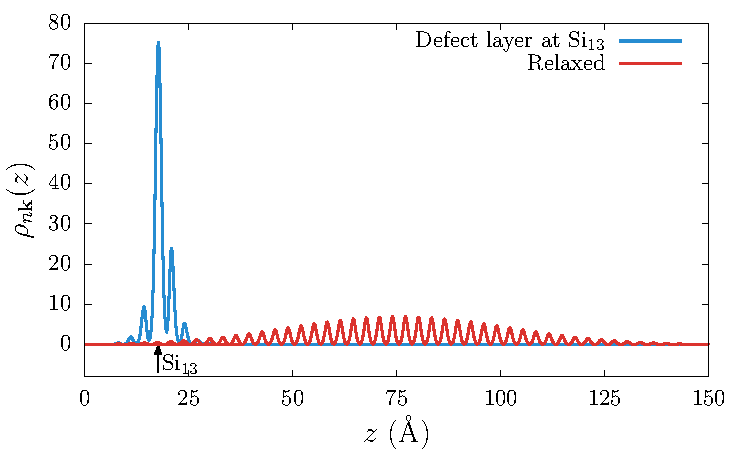
\includegraphics[width=\linewidth]{fig05}
\caption{
The planar-integrated electron density $\rho_{n\mathbf{k}}(z)$ as a function of
depth for the relaxed slab and the defective slab with a defect layer at
Si$_{13}$. The small black arrow indicates the $z$ position of Si$_{13}$.
}
\label{fig:defect}
\end{figure}

Our results clearly show that the calculated signals are well within the
detection range of lock-in techniques; thus, depth-probing and defect detection
should be possible with this method. Experimentally, it is not easy to obtain a
sample as the ones described above. However, a feasible test material could be
synthesized with a buried monolayer comprised of some other material, in lieu of
having a layer of atoms displaced from their equilibrium position. We emphasize
that even though the specifics of our results depend on the excitation, the
model can be applied to an arbitrary perturbation that produces a strain wave,
and is not necessarily exclusive to CAP experiments. Although the type of defect
layer presented here (created via uniform atomic displacement) would be
difficult to recreate experimentally, it provides an effective test platform for
our method. Localized defects, such as those produced by doping, require very
large unit cells that increase the computational demand of the calculations. As
is, our method should be effective at discovering buried interfaces, even
between different materials.

%%%%%%%%%%%%%%%%%%%%%%%%%%%%%%%%%%%%%%%%%%%%%%%%%%%%%%%%%%%%%%%%%%%%%%%%%%%%%%%%
%%%%%%%%%%%%%%%%%%%%%%%%%%%%%%%%%%%%%%%%%%%%%%%%%%%%%%%%%%%%%%%%%%%%%%%%%%%%%%%%

\section{Conclusions}\label{sec:conc}

Overall, our method for modeling the atomic displacement in a crystalline slab
induced by an advancing strain wave proves to be effective at discerning buried
defect layers. The strain wave is obtained by using realistic material constants
and beam parameters; thus, the atomic displacement is an accurate representation
of what might occur with a strain wave from a CAP experiment. The calculated
difference reflectance spectrum for our Si(111)(1$\times$1):H test system yields
a unique  peak in the 2.5--3.0\,eV energy range that acts as a defect signature,
allowing us to accurately pinpoint the defect layer depth.

Although the model presented here is a significant advancement over our previous
work \cite{andersonPSSB18} due to the more accurate representation of the strain
wave, we have yet to incorporate the interference effects that occur as the
probe light enters the material and interacts with the strain wave, and
undergoes multiple reflections before exiting the material. This would require
either a much larger slab, so that the atoms displaced by the strain wave could
be more localized, or the use of another material with constants that lead to a
much narrower strain wave. Larger slabs lead to significantly larger
computational expense; therefore, we consider that there may be other materials
that could produce very localized strain waves, where the disordered region can
be clearly isolated from the remainder of the unperturbed material. The
development of such a model would essentially complete our proposed \emph{ab
initio} description of CAP spectroscopy, and should be achievable in the near
future.

%%%%%%%%%%%%%%%%%%%%%%%%%%%%%%%%%%%%%%%%%%%%%%%%%%%%%%%%%%%%%%%%%%%%%%%%%%%%%%%%
%%%%%%%%%%%%%%%%%%%%%%%%%%%%%%%%%%%%%%%%%%%%%%%%%%%%%%%%%%%%%%%%%%%%%%%%%%%%%%%%

\section{Acknowledgements}
Ram\'on Carriles and Bernardo S. Mendoza thank the \emph{Red Nanociencias y
Nanotecnolog\'ia} of Mexico for partial financial support, and Bernardo S.
Mendoza acknowledges CONACYT-Mexico research grant A1-S-9410.

\bibliography{refs}
\bibliographystyle{apsrev4-1}

\end{document}
